\section{Experiment}
To confirm that NaaA works widely with machine learning tasks,
we confirm our method of supervised learning tasks as well as reinforcement learning tasks.
As supervised learning tasks, we use typical machine learning tasks such as image classification
using MNIST, CIFER-10, and SVHN.

As reinforcement tasks, we confirm single- and multi-agent environment.
The single-agent environment is from OpenAI gym.
We confirm the result using a simple reinforcement task: CartPole.
In multi-agent, we use ViZDoom, a 3D environment for reinforcement learning.

\subsection{Classification}
In the classification task, we experiment with our method using several standard datasets: MNIST, CIFER-10, and SVHN.
As a method of comparison, we compare baseline (vanilla feed-forward neural network) and DropConnect.
In a hyperparameter setting, we set $\epsilon = 0.2$, which means that the agent randomly masks the weights in 0.2 of the chance rate, 
and playing the auction game in 0.8 of chance rate.
Table \ref{tbl:result} presents our framework of NaaA complements disadvantage of DropConnect.
It randomly drops the weight completely, and does not consider implicit counterfactual return of units.

\subsection{Single-agent RL}
Next, we set the single-agent reinforcement learning task.
We used the CartPole task from OpenAI gym with visual input.
In this setting, the agent must balance a pole while moving a cart.
There is much non-useful information related to the image. For that reason, pruning the pixels is important.
The result demonstrates that our method improves the standard RL.

\subsection{Multi-agent RL}
The additional feature of NaaA is credit assignment for reward distribution, 
meaning that if the neural network is divided into multiple agents, it works by playing the auction game.
We confirmed that additional agents complement the main player using ViZDoom, an environment for Doom.
A player in Doom environment should seek the enemy in the map, and then defeat the enemy.
Because ViZDoom provides several maps, we used ViZDoom.

\subsubsection{Setup}
We used a scenario based on Defend the Center (DtC), provided by ViZDoom platform.
In DtC, players are placed in the center of a field of circle. They attack enemies that come from the wall.
The game has two players: a main player and a cameraman.
Alhough the main player can attack the enemy with bullets, 
the cameraman has no way to attack, and only scouts for the enemy.
The action space for the main player is the combination of \{ attack, turn left, turn right \}. Therefore, the total number of actions is $2^3 = 8$.
The cameraman has two possible actions: \{ turn left, turn right \}.
Although the players can only change direction, they cannot move on the field.
The enemy will die if have the attack (bullet) from the main player once.
As a default on an episode, the ammunition amount is 26.
The main player will die if under attack from the enemy to the extent that health becomes 0.
The cameraman will not die if attacked by the enemy.
The episode will terminate when the maim player dies, or after 525 steps have elapsed.

DtC is standard scenario prepared using the ViZDoom platform.
In DtC, up to five enemies can exist at the same time. 
The main player will receive a reward every time the enemy is defeated.
After the enemy dies, the player receives 1; the player receives -1 if killed.

\subsubsection{Model}
We compared three models: the proposed method and two comparison targets.

{\em Baseline} DQN without communication. The main player learns standard DQN with the perspective that the player is viewing.
Because the cameraman does not learn, the player continues to move randomly.

{\em Comm} DQN with communication. The main player learns DQN with two perspectives: the player's own and the cameraman's.
The communication vector is learned with a feed-forward neural network. The method is inspired by Commnet.

{\em NaaA} The proposed method. The main player learns DQN with two perspectives: the player's own and the cameraman's.
The transmission of reward and communication are performed using the proposed method.

\subsubsection{Results}
Training is performed in 10 million steps.
Figure \ref{fig:learning_curve} presents that our model NaaA outperforms CommNet.
Improvement is achieved by a distribution of rewards and adaptive dropout.
We confirmed that the cameraman sees the enemy through an episode.
This can be interpreted as the cameraman reporting the enemy position.
In addition to seeing the enemy, the cameraman sees the area behind of main player several times.
This action enables the cameraman to observe attacks from the enemy while seizing a better relative position.

For further interpretation of the result, 
we present visualization of the revenue that the agent earned in Figure \ref{fig:vis} as a heatmap.
The background picture is a screen in Doom taken at the moment when the filter in CNN is mostly activated.
Figure \ref{fig:vis}(a) shows what the agent sees at the top and center of the screen.
The center corresponds to a position with the enemy appearing far away.
The top corresponds to a position with the enemy coming closer.
Figure \ref{fig:vis}(b) shows that the agent sees the pistol.

%\begin{figure*}[t]
%\begin{center}
%\begin{minipage}[t]{0.45\textwidth}
%\centering
%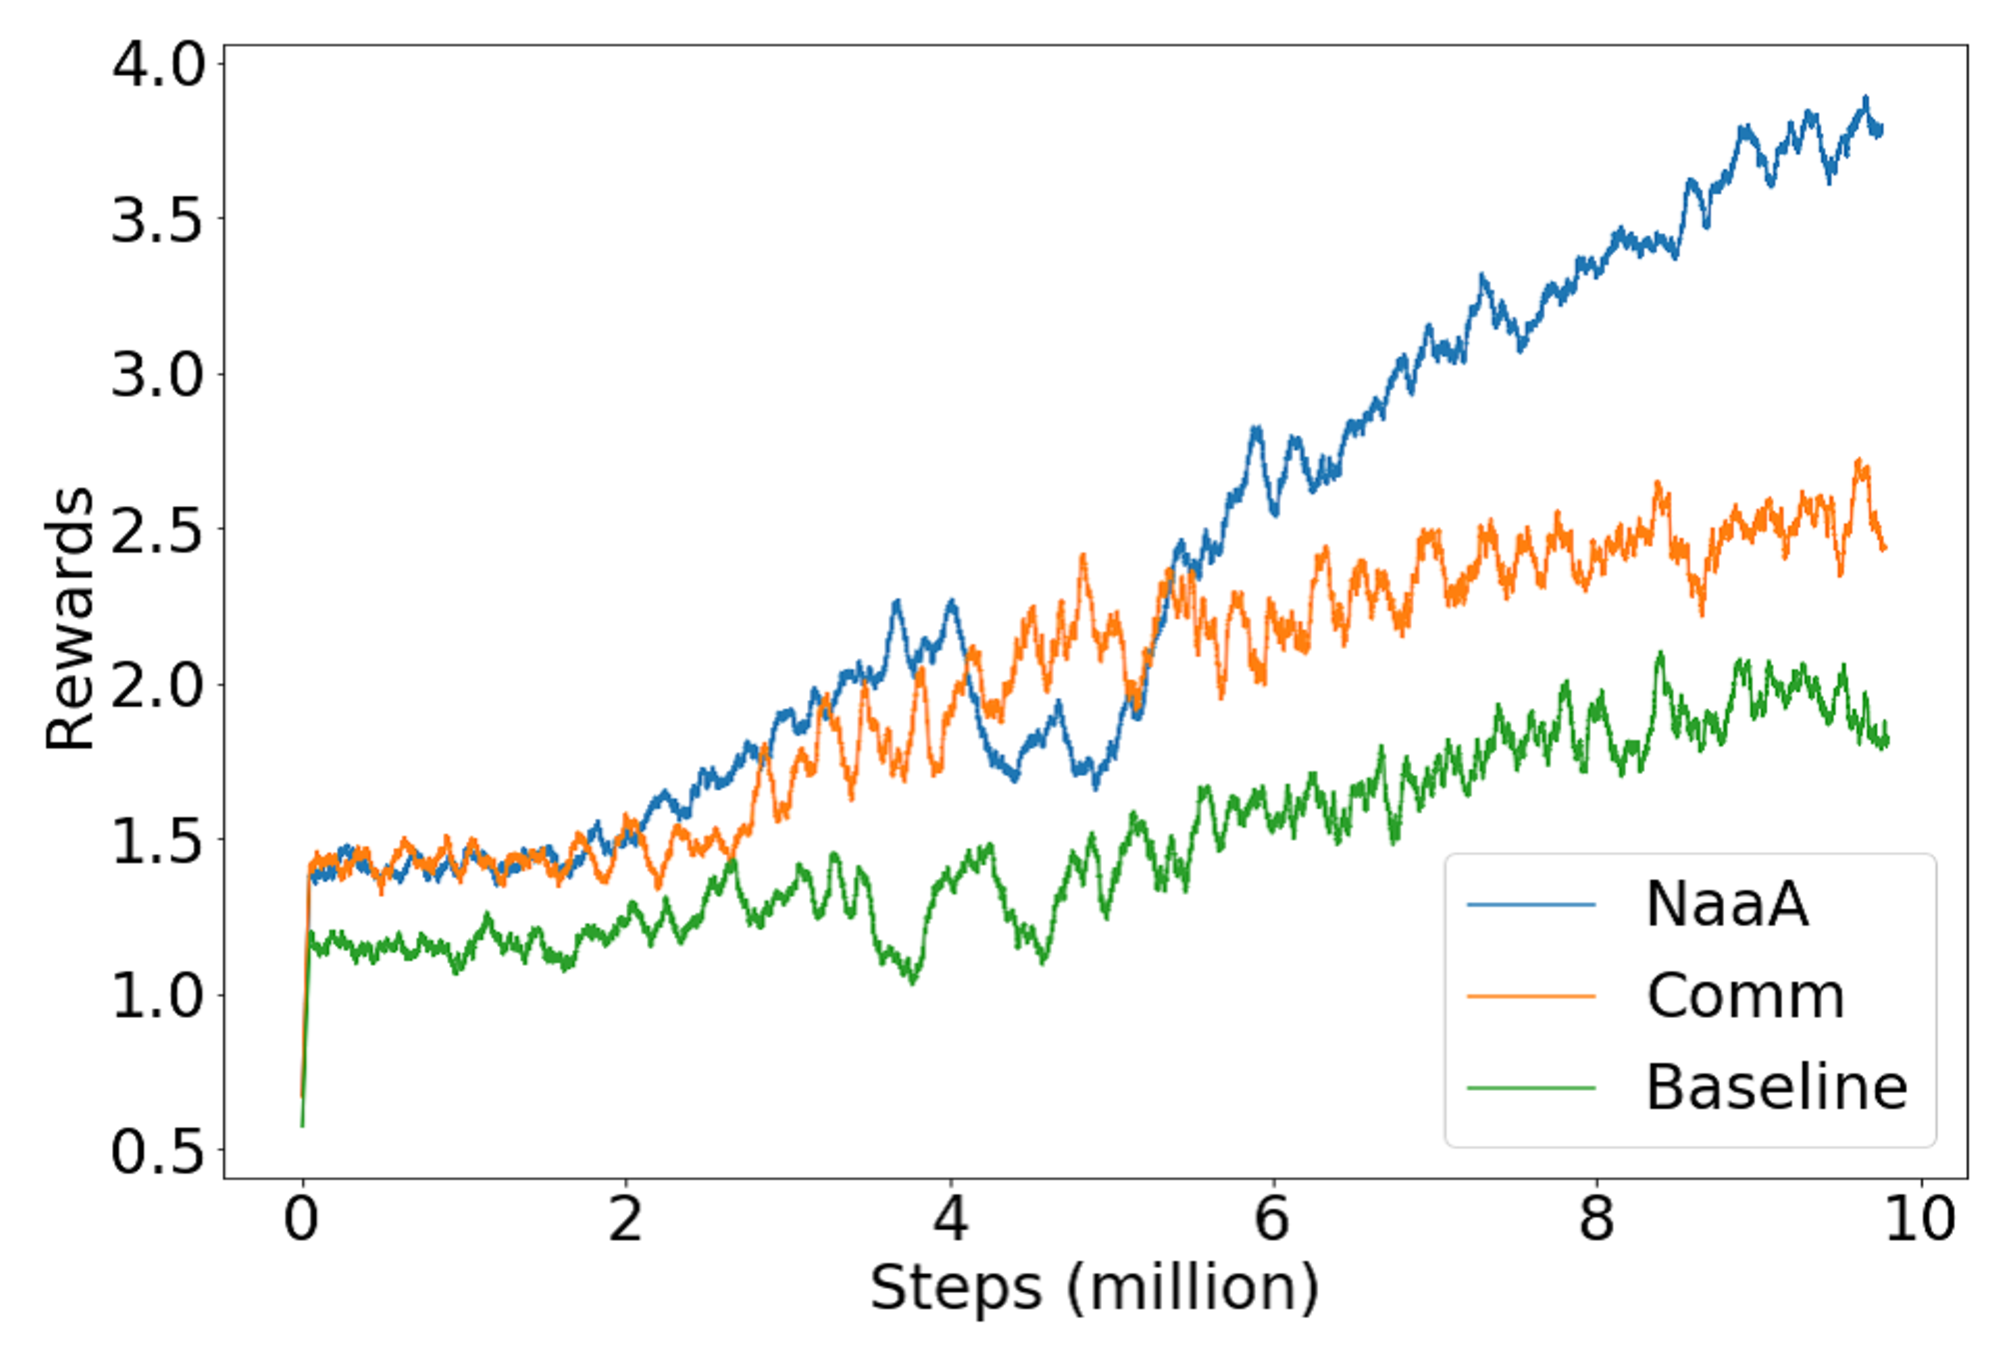
\includegraphics[width=\textwidth]{img/learning_curve_trim.eps}
%\caption{
%Learning curve for the multi-agent task of VizDoom. 
%Our method based on NaaA outperforms other two methods, baseline and CommNet \citep{sukhbaatar2016learning}.
%}
%\label{fig:learning_curve}
%\end{minipage}
%\,\,
%\begin{minipage}[t]{0.53\textwidth}
%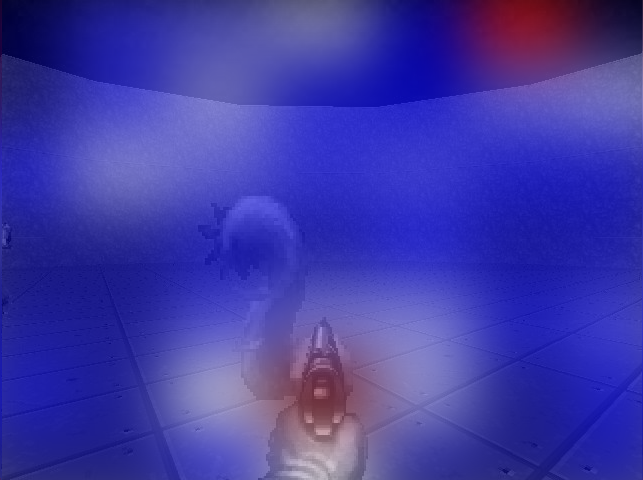
\includegraphics[width=0.49\textwidth]{img/vis2.eps}
%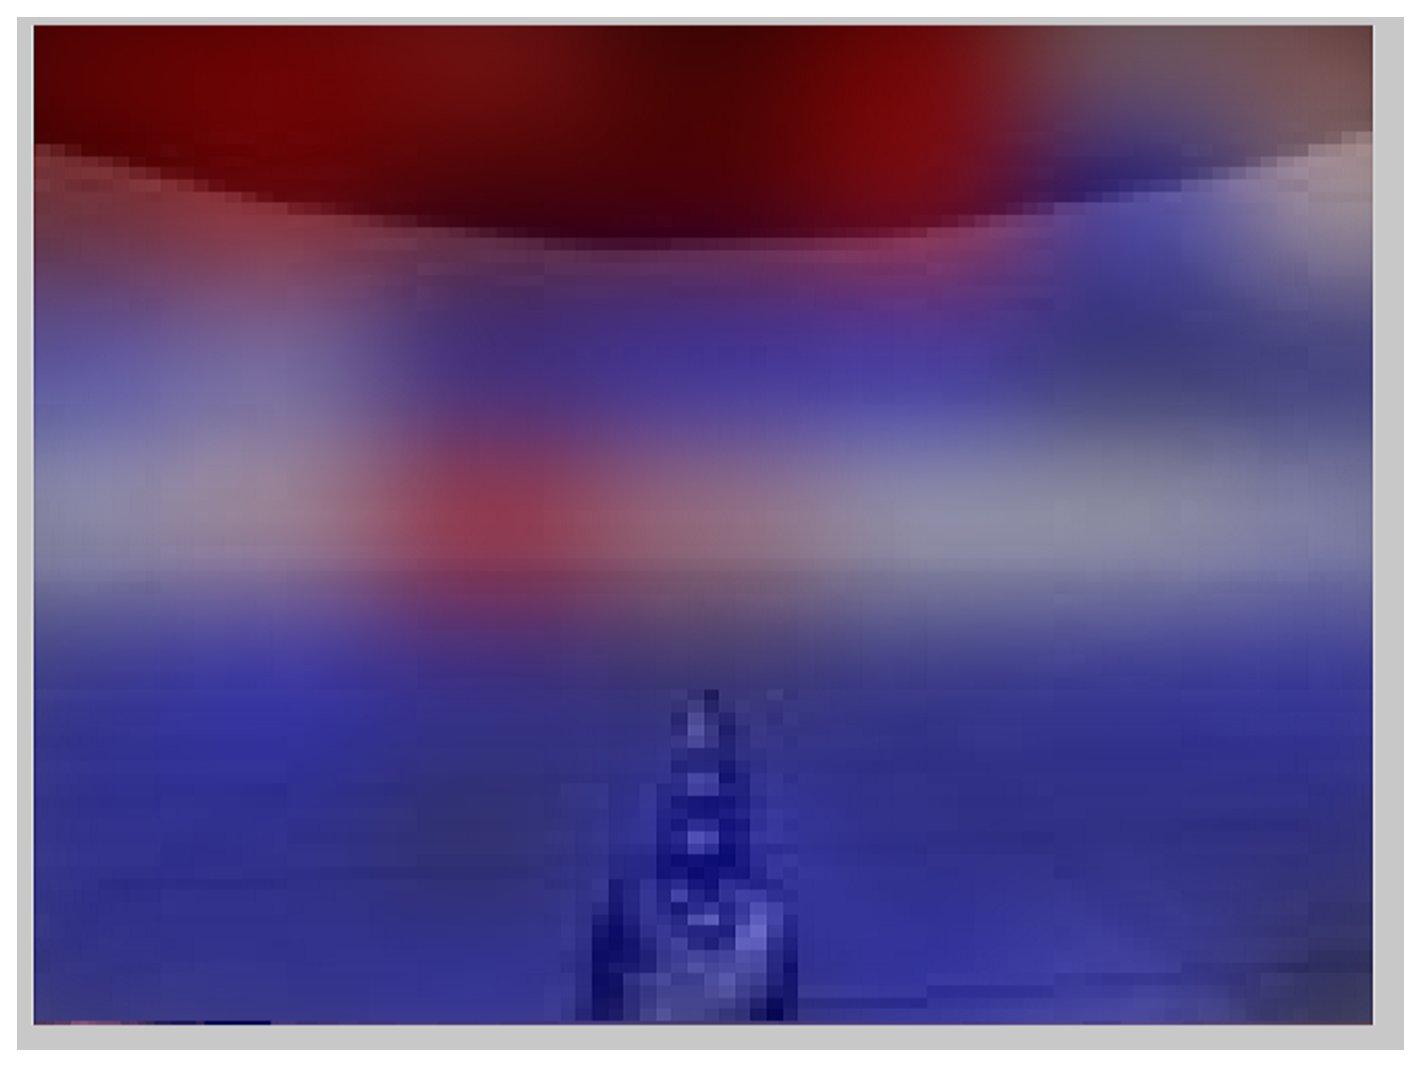
\includegraphics[width=0.49\textwidth]{img/vis1.eps}
%\caption{
%Reward visualization tells us what the cameraman sees. 
%(a) cameraman sees the point which enemy appear and come closer.
%(b) cameraman sees the pistol.
%}
%\label{fig:vis}
%\end{minipage}
%\end{center}
%\end{figure*}
%
\begin{figure*}[t]
\centering
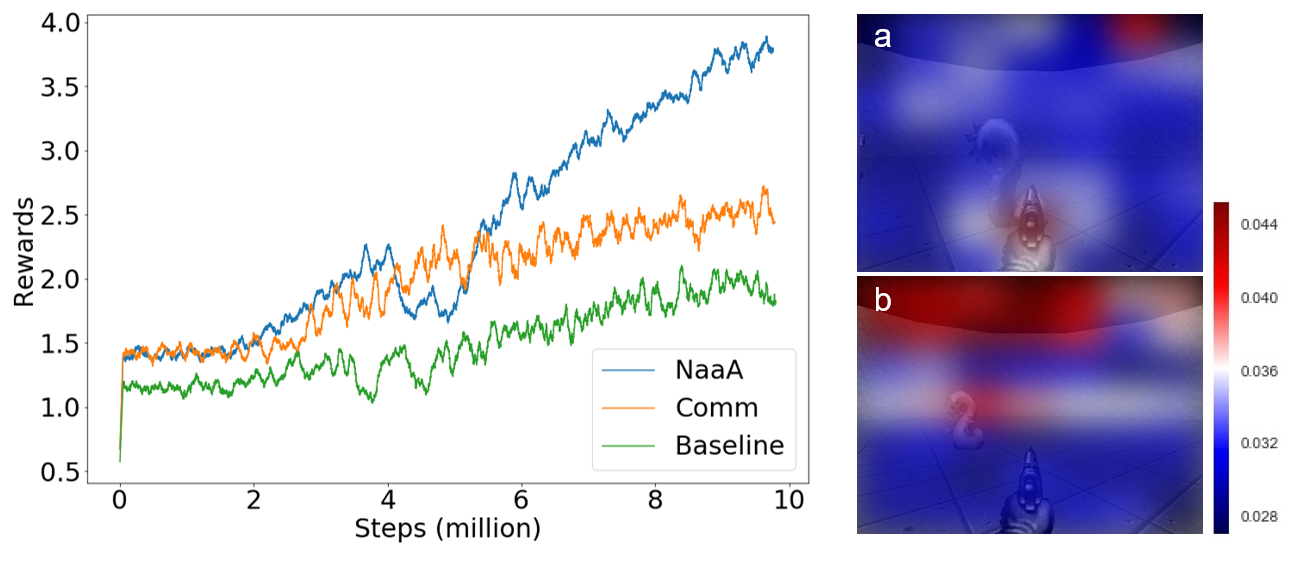
\includegraphics[width=\linewidth]{img/lc_vis.eps}
\caption{
	\textbf{Left:}
		Learning curve for the multi-agent task of VizDoom. 
		Our method based on NaaA outperforms the other two methods: baseline and Comm DQN.
	\textbf{Right:} 
		Reward visualization shows us what the cameraman sees:
		(a) The cameraman sees the point which enemy appear and come closer.
		(b) The cameraman sees the pistol.
}
\label{fig:double}
\end{figure*}


\begin{figure*}[t]
\centering
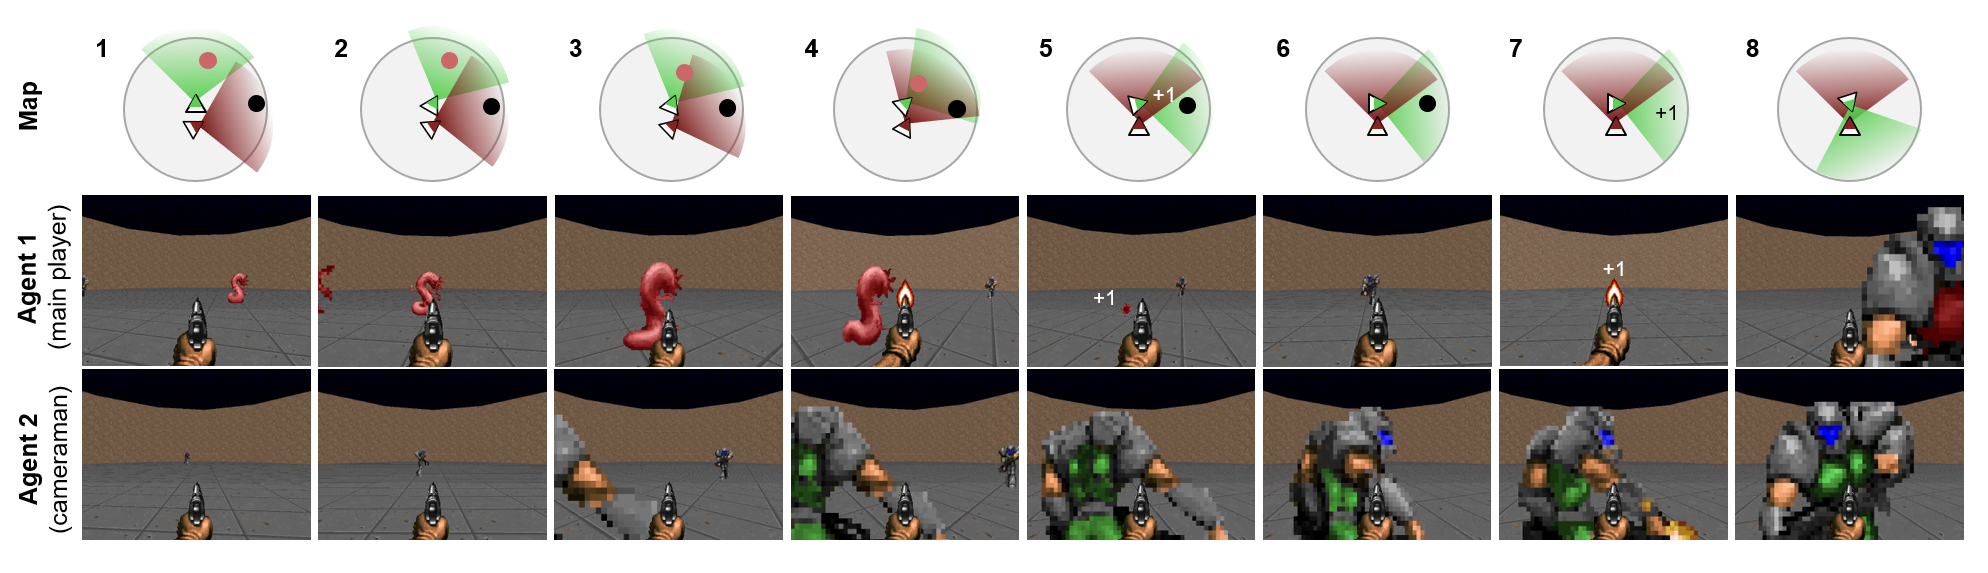
\includegraphics[width=\linewidth]{img/circleworld.eps}
\caption{
NaaA leads the agents to obtain cooperate relationship.
First, the two agents are seeing different direction, and the cameraman sells its information to the main player (\textbf{1}).
The main player who bought the information starts to turn right to find the enemy.
The cameraman who sold the information starts to turn left to seek new information by seeing dead angle of the main player (\textbf{2} and \textbf{3}).
With turning, the main player attacks the first enemy which he already saw (\textbf{4} and \textbf{5}).
After the main player finds out the enemy, he attack the enemy, and obtain the reward  (\textbf{6} and \textbf{7}).
Until the next enemy appears, the agents watch their dead area each other (\textbf{8}).
}
\label{fig:double}
\end{figure*}
%An example of sequences which the agents obtained by NaaA.
%
%NaaA によってエージェントが獲得した行動系列の例。
%	最初、二つのエージェントは異なる方向を見ており、Agent 2 は Agent 1 に対して自分が見ている方向と敵の存在を教える(1)
%		その情報を受け取った main player は、敵のいる右方向に旋回する(2,3)
%	main player は旋回しながら、すでに相手にしている敵を倒す。役目を終えた cmeraman は、counterfactual return を高めるために、すかさず main palyer の死角を見に行く。(4,5)		
%	敵を発見した main player は、敵を銃撃して倒し、リワードを獲得する(6,7)。
%	次に敵が出現するまでの間、エージェントはお互いの死角を監視しあう(8)。
%}

%訓練は1000万ステップ行われた。
%TODO: 1.スコアが高いことを言う。2.潜在変数の値段や、シグナルの活性化を見る。
